% main.tex
\documentclass[12pt]{scrreprt}
\usepackage[a4paper, margin=2.5cm]{geometry}
\usepackage{xcolor}
\usepackage{listings}
\usepackage{underscore}
\usepackage[english]{babel}
\usepackage{scrlayer-scrpage}
\usepackage{setspace}
\usepackage{titlesec}
\usepackage[utf8]{inputenc}
\usepackage{placeins}
\usepackage{float}
\usepackage{graphicx}
\usepackage{caption}    % 允许子图使用 caption
\usepackage{subcaption} 
\usepackage{array}
\usepackage{colortbl}
\usepackage{booktabs}
\usepackage[bookmarks=true]{hyperref}
\usepackage{parskip}           % 段落间距
\setlength{\parskip}{0.5em}    % 紧凑段落间距
\renewcommand{\baselinestretch}{1.05} % 行距微调

% main.tex导言区
\usepackage{titlesec}
\titleformat{\chapter}[block]
{\normalfont\huge\bfseries}{\thechapter}{1em}{}
\titleformat{\section}[block]
{\normalfont\Large\bfseries}{\thesection}{1em}{}
\titleformat{\subsection}[block]
{\normalfont\large\bfseries}{\thesubsection}{1em}{}
% 保持编号与标题的经典间距
\makeatletter
\renewcommand{\@seccntformat}[1]{\csname the#1\endcsname\quad}
\makeatother

% 现代间距系统(单位:pt)
\titlespacing*{\chapter}{0pt}{25pt}{15pt}  % 上间距25pt/下间距15pt
\titlespacing*{\section}{0pt}{15pt}{7pt}
\titlespacing*{\subsection}{0pt}{10pt}{5pt}

% 确保子章节编号
\setcounter{secnumdepth}{3}
\setcounter{tocdepth}{3} % 目录显示到三级标题

% 封面字体优化
\usepackage{anyfontsize}        % 精确字体控制
\usepackage[sfdefault]{noto}   % 现代无衬线字体(需要安装Noto Sans字体)

%refers
\usepackage[style=ieee, sorting=none, backend=biber]{biblatex}
\addbibresource{re.bib}

% Hyperref配置
\hypersetup{
    pdftitle={Software Requirement Specification},
    pdfauthor={Jean-Philippe Eisenbarth},
    pdfsubject={TeX and LaTeX},
    pdfkeywords={TeX, LaTeX, SRS, Requirements},
    colorlinks=true,
    linkcolor=blue!70!black,
    citecolor=green!60!black,
    filecolor=magenta,
    urlcolor=cyan!70!black,
    linktoc=page
}

% 全局格式设置
\setstretch{1.1}
\titleformat{\chapter}[display]
{\normalfont\huge\bfseries}{\chaptertitlename\ \thechapter}{20pt}{\Huge}
\titlespacing*{\chapter}{0pt}{-30pt}{40pt}

% 自定义命令
\newcommand{\placeholder}[1]{\textcolor{gray!70}{\textlangle\,\textit{#1}\,\textrangle}}
\newcommand{\req}[2]{\item[REQ-#1:] #2} %详见设置文件

\newcommand{\myversion}{1.0}   %在这里更改文档版本

\begin{document}

% 封面
% cover.tex
\begin{flushright}
    \vspace*{1.5cm}
    \rule{0.75\textwidth}{5pt}
    
    \vspace{1.2cm}
    \fontsize{30}{28}\selectfont
    \textbf{Detailed Design}
    
    \vspace{1.5cm}
    \fontsize{14}{16}\selectfont
    for
    
    \vspace{1cm}
    \fontsize{18}{22}\selectfont
    Design and Implementation of a Lightweight \\[0.3em]
    Education Data Bay Area (E-DBA)
    
    \vspace{1.5cm}
    \fontsize{13}{15}\selectfont
    Version \myversion\ Approved
    
    \vspace{1.8cm}
    \begin{minipage}{0.7\textwidth}
    \flushright
    \fontsize{12}{14}\selectfont
    \textbf{Prepared by:} \\
    Taian Yu (FULL)\quad Yolanda Yin (FULL) \\
    Justin Zhang (FULL)\quad Aaron Liu (FULL) \\
    Steven Luo (FULL)\quad Younger Yang (FULL)
    \end{minipage}
    
    \vspace{1.2cm}
    \fontsize{14}{16}\selectfont
    Group C01
    
    \vspace{2cm}
    \today
\end{flushright}

% 目录
\tableofcontents

%迭代历史
\chapter*{Revision History}
\begin{center}
    \rowcolors{2}{gray!15}{white} % 设置表格隔行颜色
    \begin{tabular}{>{\raggedright\arraybackslash}p{3.5cm}
                    >{\raggedright\arraybackslash}p{3cm}
                    >{\raggedright\arraybackslash}p{5cm}
                    >{\centering\arraybackslash}p{2cm}}
        \toprule[1.5pt]
        \rowcolor{gray!30} % 表头颜色
        \textbf{Name} & \textbf{Date} & \textbf{Reason For Changes} & \textbf{Version}\\
        \midrule
        All Members & 9 April & Create the document & 1.0\\
        \bottomrule[1.5pt]
    \end{tabular}
\end{center}



\chapter{Overview}
\section{Project Description}

This project focuses on designing the architecture for five core subsystems: User, Restructure, Service, Others, and Data. Each subsystem will have its own architecture, UI layers, and persistent data tables to ensure scalability and organization. The design aims to minimize interdependencies between subsystems, allowing for independent development and seamless integration.

Detailed design documentation will include use case diagrams, class diagrams, and explicit system component relationships to ensure autonomous operation and integration between subsystems.

\section{References}

\begin{itemize}
  \item Software Requirements Specification (SRS)
  \item UI Design Document
  \item Architecture Design Document
\end{itemize}

\section{Design Purpose}

The design aims to establish a modular structure enhancing maintainability, scalability, and separation of concerns across subsystems. Dedicated subsystems for different architectural layers and data tables minimize associations across boundaries, ensuring efficient data flow and simplified future extensions.


\chapter{Overall description}
\section{Class diagram}
\begin{figure}[H]
    \centering
    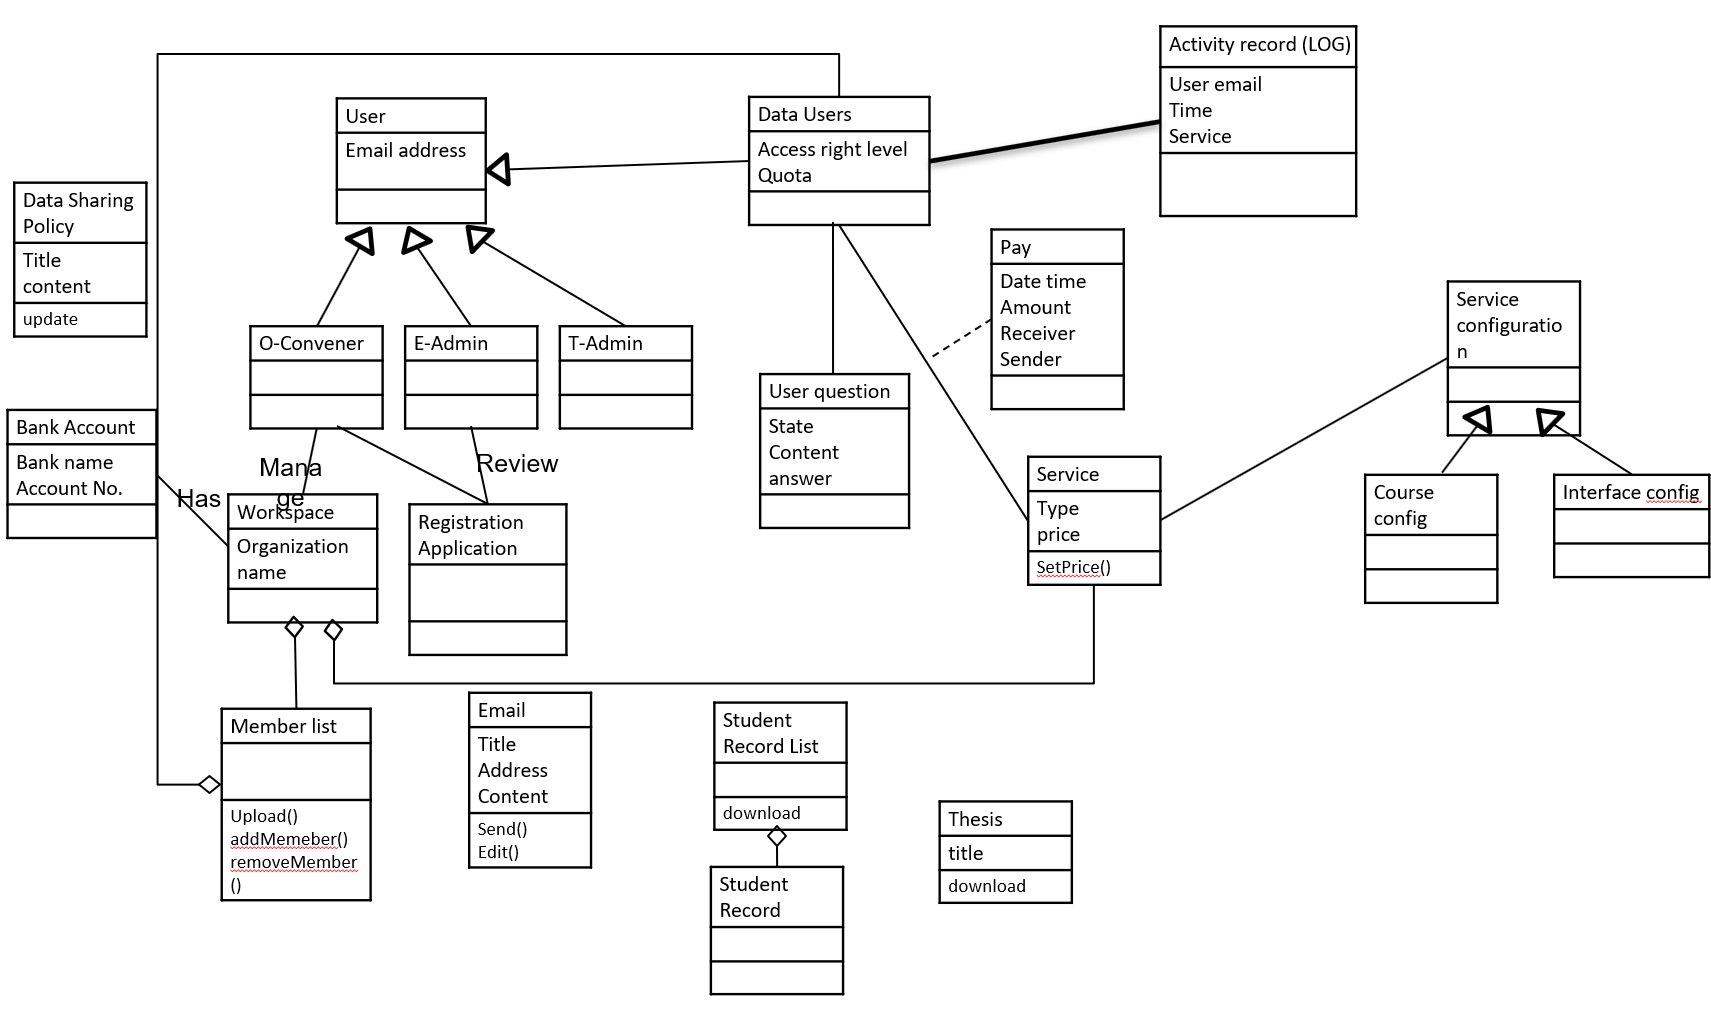
\includegraphics[width=0.75\linewidth]{picture/2-1/2-1-1.jpg}
    \caption{Class diagram}
    \label{fig:enter-label}
\end{figure} 

\section{Refinements}

\textbf{Splitting overly complex classes, merging similarly functioning classes, and adjusting inheritance and association relationships between classes.}

\begin{itemize}
    \item \textbf{Identifying features:} Clarify the core functionality and properties of each class. By analyzing the requirements and functional modules, we identify the key characteristics of each class and translate them into specific properties and methods.
    \item \textbf{Specifying Visibility and Constraints:} We set the appropriate level of access (such as public, private, or protected) for the properties and methods of each class to ensure the encapsulation and security of the data.
    \item \textbf{Constraints between classes:} For example, polymorphism through interfaces, or inheritance of classes to restrict how certain behaviors can be implemented.
\end{itemize}

\chapter{Detailed design}
\section{Class diagram}

\begin{figure}[H]
    \centering
    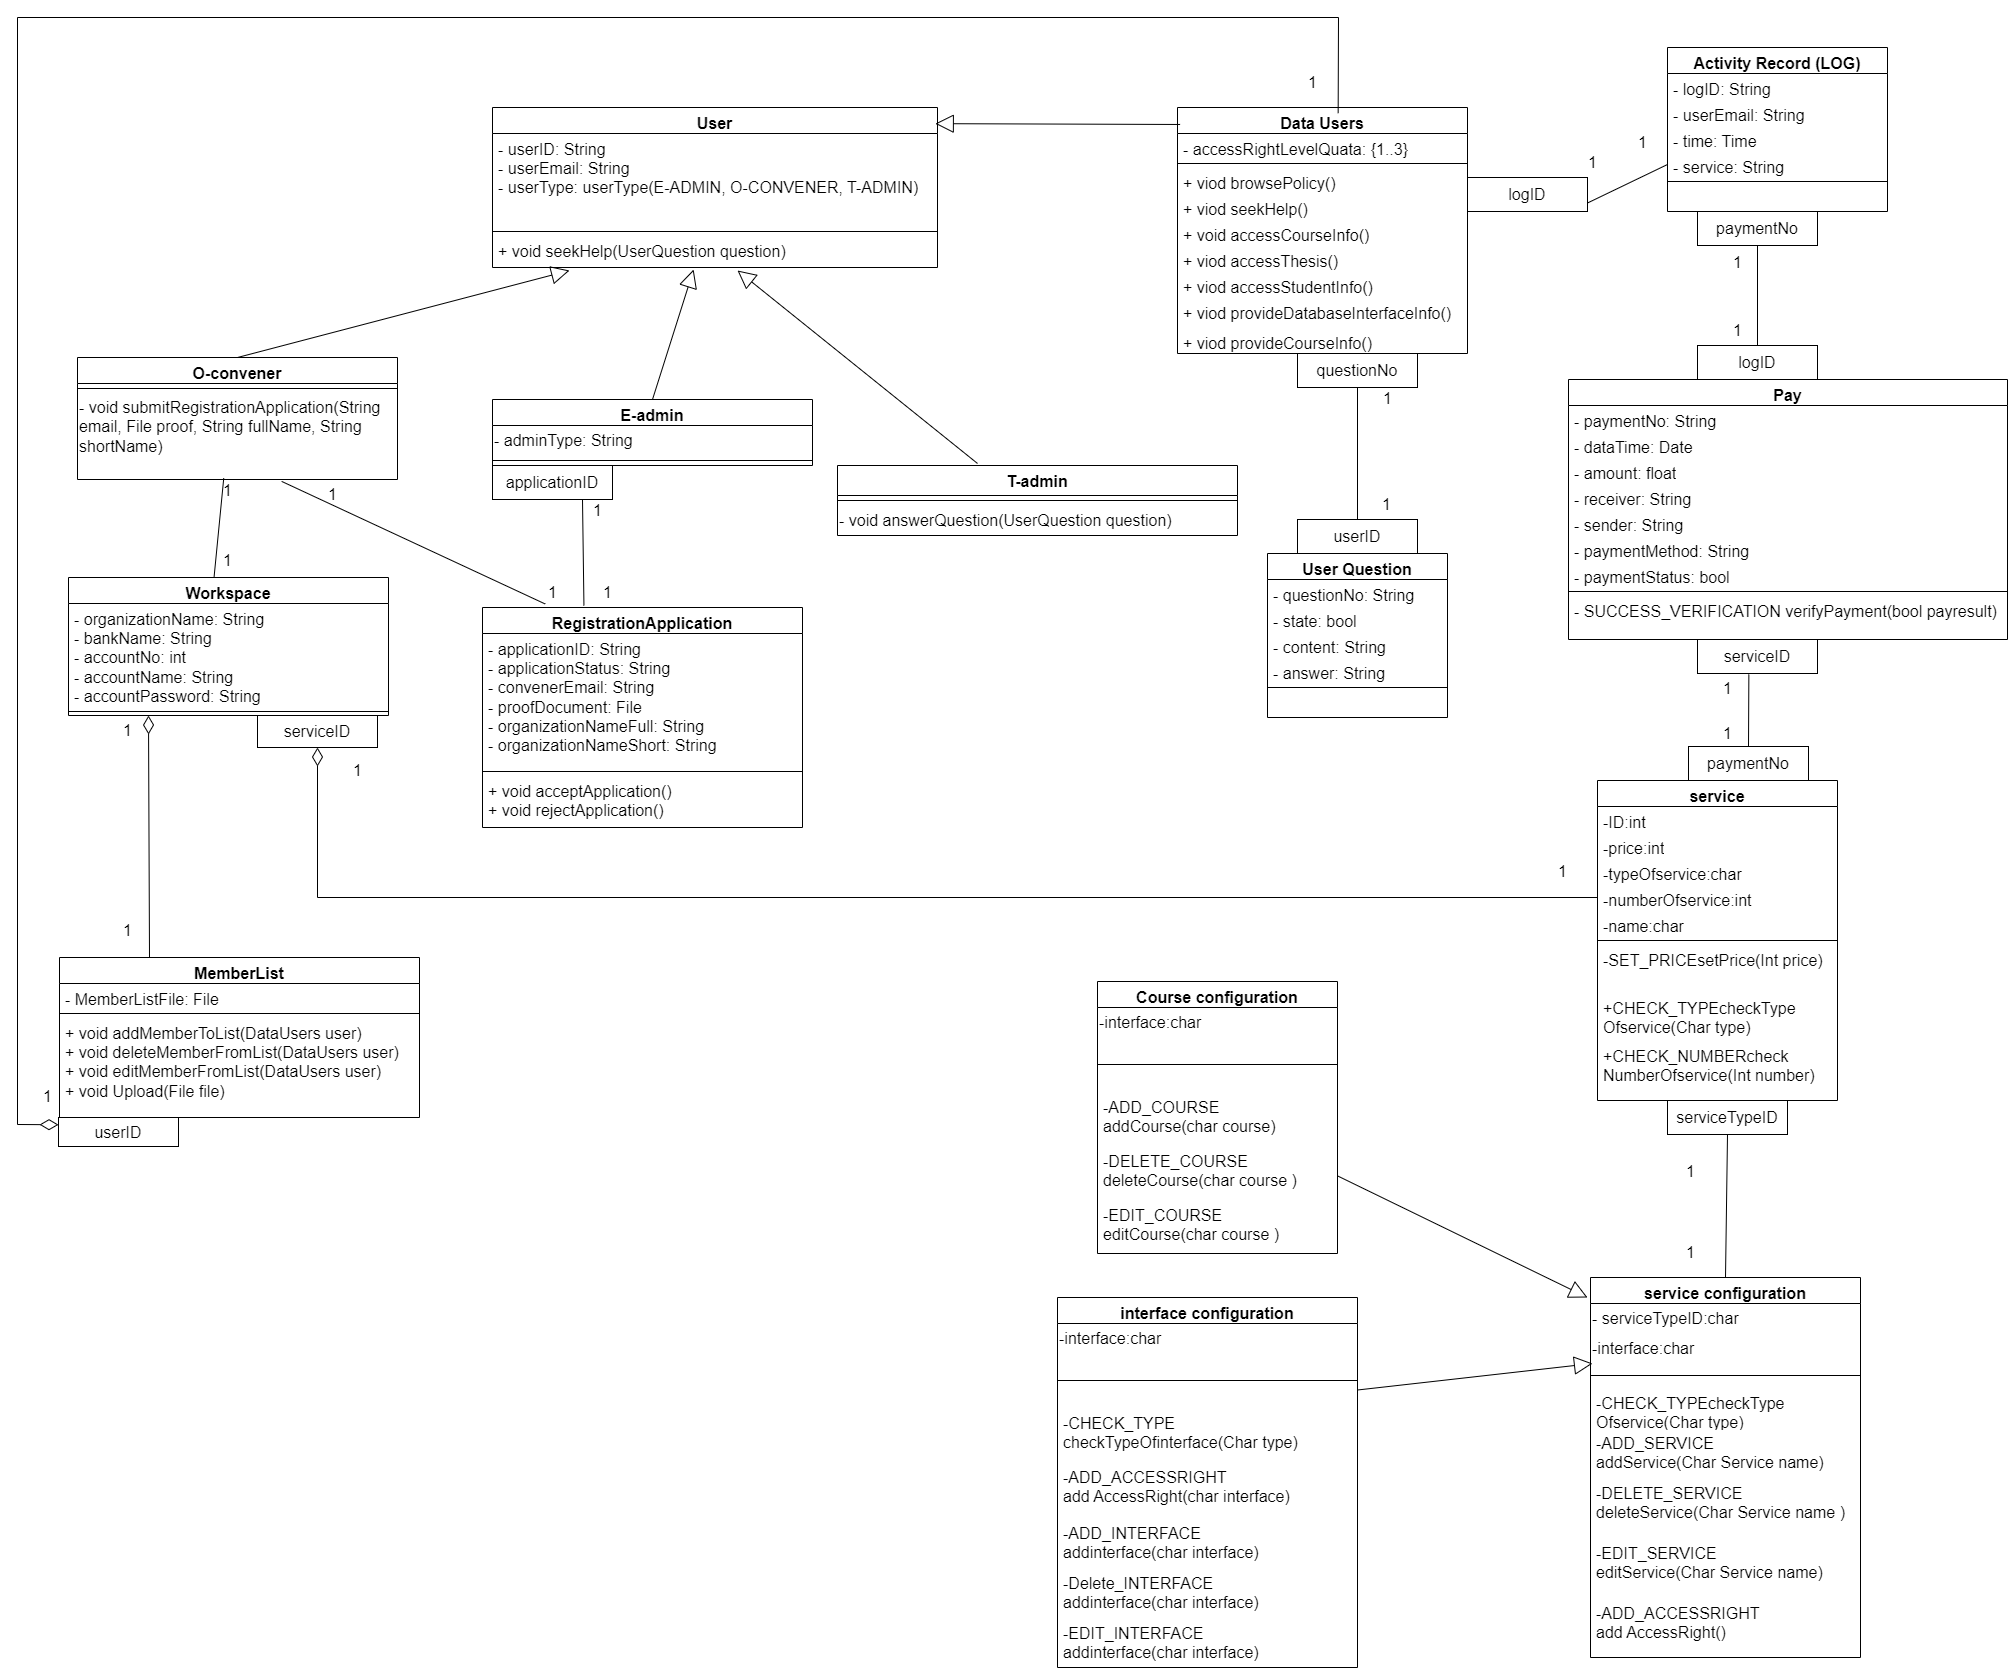
\includegraphics[width=1\linewidth]{picture/3-1/3-1-2A.jpg}
    \caption{Restructure Class}
    \label{fig:enter-label}
\end{figure}

\begin{figure}[H]
    \centering
    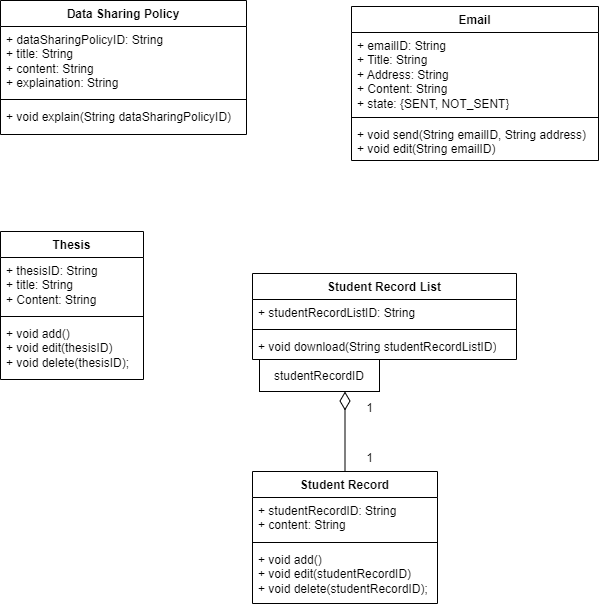
\includegraphics[width=0.75\linewidth]{picture/3-1/3-1-2B.jpg}
    \caption{Restructure Class}
    \label{fig:enter-label}
\end{figure}

Compared to the previous class diagram, the following relationships have been added first:
\begin{itemize}
    \item O-convener and Workspace are a one-to-one relationship.
    \item O-convener and Registration Application are a one-to-one relationship.
    \item E-Admin and Registration Application are a one-to-many relationship.
    \item Workspace and Member List are a one-to-one relationship.
    \item Workspace and Service are a one-to-many relationship.
    \item Member List and Data Users are a one-to-many relationship.
    \item Data Users and User Questions are a many-to-many relationship.
    \item Data Users and Activity Records are a one-to-many relationship.
    \item Service and Service Configuration are a one-to-many relationship.
    \item Implement an association Class \texttt{Pay} as a class. Among them, Data Users and \texttt{Pay} are a many-to-many relationship, while \texttt{Pay} and Service are a many-to-many relationship.
\end{itemize}

After reconstruction, the relationship changes as follows:
\begin{itemize}
    \item Collapse the \texttt{BankAccount} class into attributes of Workspace.
    \item The following relationships use Use Qualifier to reduce multiplicity:
    \begin{itemize}
        \item E-Admin and Registration Application
        \item Member List and Data Users
        \item Workspace and Service
        \item Data Users and User Questions
        \item Data Users and Activity Records
        \item Service and Service Configuration
        \item Data Users and Pay
        \item Pay and Service
    \end{itemize}
\end{itemize}


\section{User}

\subsection{User}

\begin{figure}[H]
    \centering
    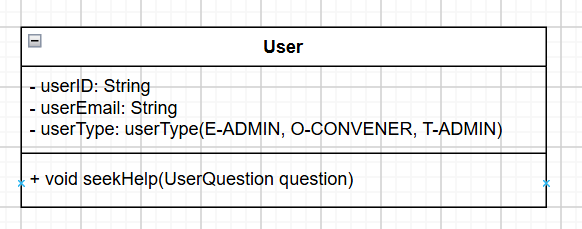
\includegraphics[width=0.7\linewidth]{picture/3-2/3-2-1.png}
    \caption{User}
    \label{fig:enter-label}
\end{figure}

\textbf{Explanations}
\begin{itemize}
    \item The additional attribute \texttt{userType: char} determines the role of the user:
    \begin{itemize}
        \item \texttt{E-admin} (Event Administrator)
        \item \texttt{O-convener} (Organizing Convener)
        \item \texttt{T-admin} (Technical Administrator)
    \end{itemize}
    \item The operation \texttt{seekHelp()} allows users to post technical help requests to \texttt{T-admins}.
\end{itemize}

\textbf{Constraints} \\
TBD

\subsection{T-Admin}
\begin{figure}[H]
    \centering
    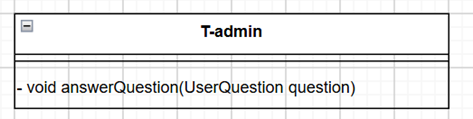
\includegraphics[width=0.7\linewidth]{picture/3-2/3-2-2.png}
    \caption{T-Admin}
    \label{fig:enter-label}
\end{figure}

\textbf{Explanations}
\begin{itemize}
    \item The operation \texttt{answerQuestion()} allows the \texttt{T-admin} to answer help requests.
\end{itemize}

\textbf{Constraints} \\
TBD

\subsection{E-Admin}
\begin{figure}[H]
    \centering
    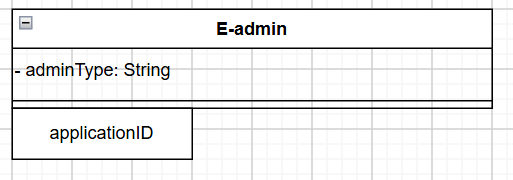
\includegraphics[width=0.7\linewidth]{picture/3-2/3-2-3.png}
    \caption{E-Admin}
    \label{fig:enter-label}
\end{figure}

\textbf{Explanations}
\begin{itemize}
    \item The attribute \texttt{adminType: String} indicates whether the user is a(n) \texttt{E-admin} or \texttt{Senior E-admin}.
\end{itemize}

\textbf{Constraints} \\
TBD

\subsection{O-Convener}
\begin{figure}[H]
    \centering
    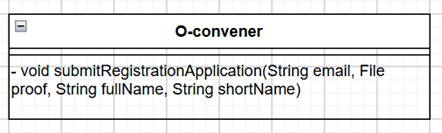
\includegraphics[width=0.7\linewidth]{picture/3-2/3-2-4.png}
    \caption{E-Admin}
    \label{fig:enter-label}
\end{figure}

\textbf{Explanations}
\begin{itemize}
    \item For the \texttt{submitRegistrationApplication} method:
    \begin{itemize}
        \item \textbf{Pre-condition:}
        \begin{itemize}
            \item email, proof, fullName, and shortName cannot be null
            \item email must be in a valid email format
            \item proof must be in a valid PDF format
        \end{itemize}
        \item \textbf{Post-condition:}
        \begin{itemize}
            \item If email is already registered, return \texttt{EMAIL\_ALREADY\_REGISTERED}
            \item Otherwise, a new registration application is created and sent to the E-admin for review, return \texttt{SUBMISSION\_SUCCESSFUL}
        \end{itemize}
    \end{itemize}
\end{itemize}

\textbf{Constraints} \\
TBD

\subsection{Workspace}
\begin{figure}[H]
    \centering
    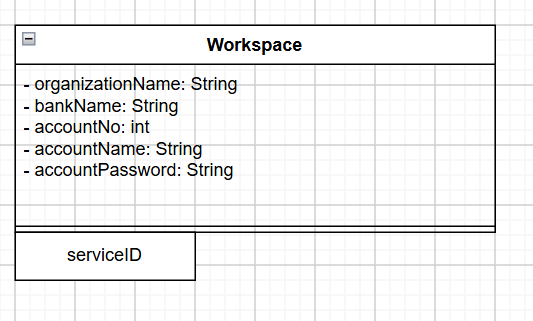
\includegraphics[width=0.7\linewidth]{picture/3-2/3-2-5.png}
    \caption{E-Admin}
    \label{fig:enter-label}
\end{figure}

\textbf{Explanations}
\begin{itemize}
    \item The attribute \texttt{bankName} indicates the name from where the account was opened.
    \item The attribute \texttt{accountNo} indicates the account ID.
    \item The attribute \texttt{accountName} indicates the name the account belongs to.
\end{itemize}

\textbf{Constraints} \\
TBD

\subsection{Registration Application}
\begin{figure}[H]
    \centering
    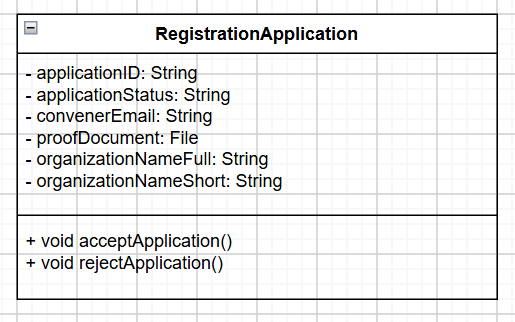
\includegraphics[width=0.7\linewidth]{picture/3-2/3-2-6.png}
    \caption{E-Admin}
    \label{fig:enter-label}
\end{figure}

\textbf{Explanations}
\begin{itemize}
    \item The additional attribute \texttt{applicationStatus: String} indicates whether the application passes the review of both the E-admin and Senior-admin.
    \item The attribute \texttt{convenerEmail} is required by E-DBA for contacting and notifying purposes.
    \item The attribute \texttt{proofDocument} is a PDF file as proofing documentation.
    \item The operation \texttt{acceptApplication()} changes \texttt{applicationStatus}.
    \item The operation \texttt{rejectApplication()} changes \texttt{applicationStatus}.
\end{itemize}

\textbf{Constraints} \\
TBD

\subsection{Member List}
\begin{figure}[H]
    \centering
    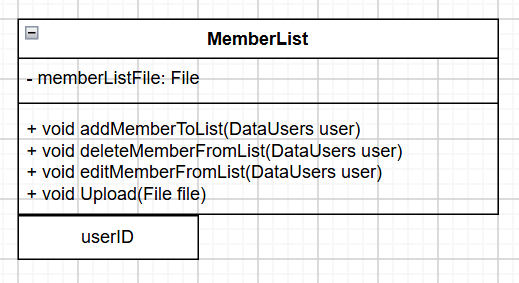
\includegraphics[width=0.7\linewidth]{picture/3-2/3-2-7.png}
    \caption{E-Admin}
    \label{fig:enter-label}
\end{figure}

\textbf{Explanations}
\begin{itemize}
    \item The additional attribute \texttt{memberListFile: File} is an Excel format file that includes the list of members in the organization, including information about name, email, access rights, and quota limits.
\end{itemize}

\textbf{Constraints} \\
TBD

\section{Service}

\subsection{Service}
\begin{figure}[H]
    \centering
    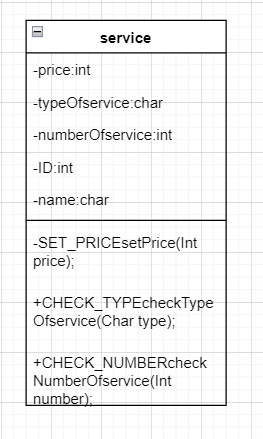
\includegraphics[width=0.3\linewidth]{picture/3-4/3-4-1.png}
    \caption{Service}
    \label{fig:enter-label}
\end{figure}

\textbf{Explanations}
\begin{itemize}
    \item \texttt{- price: int} is the price of the service
    \item \texttt{- typeOfservice: char} is the type of the service
    \item \texttt{- numberOfservice: int} is the number of the service
    \item \texttt{- ID: int} is the ID of the service
    \item \texttt{- name: char} is the name of the service
\end{itemize}

\begin{itemize}
    \item \texttt{+ SET\_PRICEsetPrice(int price)} can let the admin set the price of the service
    \item \texttt{+ CHECK\_TYPEcheckTypeOfservice(char type)} can let the admin and user see the different types of service
    \item \texttt{+ CHECK\_NUMBERcheckNumberOfservice(int number)} can let the admin and user see the number of services
\end{itemize}

\textbf{Constraints} \\
\begin{itemize}
    \item \texttt{- SET\_PRICEsetPrice(int price)} is the pre-condition. The price must be more than 0.
\end{itemize}


\subsection{Service Configuration}
\begin{figure}[H]
    \centering
    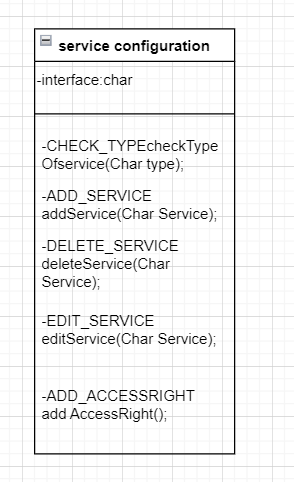
\includegraphics[width=0.3\linewidth]{picture/3-4/3-4-2.png}
    \caption{Service Configuration}
    \label{fig:enter-label}
\end{figure}

\textbf{Explanations}
\begin{itemize}
    \item \texttt{- interface: char} is the interface of service configuration
    \item \texttt{- CHECK\_TYPEcheckTypeOfservice(char type)} is to check the type of service that needs to be configured
    \item \texttt{- ADD\_SERVICEaddService(char Service name)} is to add a new service that needs to be configured
    \item \texttt{- DELETE\_SERVICEdeleteService(char Service name)} is to delete the service
    \item \texttt{- EDIT\_SERVICEeditService(char Service name)} is to edit the service that needs to be configured
    \item \texttt{- ADD\_ACCESSRIGHTaddAccessRight()} is to add the right for users to access the service
\end{itemize}

\textbf{Constraints} \\
TBD


\subsection{Course Configuration}
\begin{figure}[H]
    \centering
    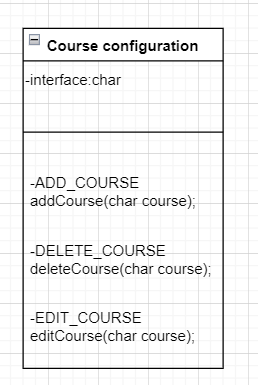
\includegraphics[width=0.3\linewidth]{picture/3-4/3-4-3.png}
    \caption{Course Configuration}
    \label{fig:enter-label}
\end{figure}

\textbf{Explanations}
\begin{itemize}
    \item \texttt{- interface: char} is the interface of course configuration
    \item \texttt{- ADD\_COURSEaddCourse(char Course)} is to add a new course that needs to be configured
    \item \texttt{- DELETE\_COURSEdeleteCourse(char Course)} is to delete the course
    \item \texttt{- EDIT\_COURSEeditCourse(char Course)} is to edit the course that needs to be configured
\end{itemize}

\textbf{Constraints} \\
TBD

\subsection{Interface Configuration}
\begin{figure}[H]
    \centering
    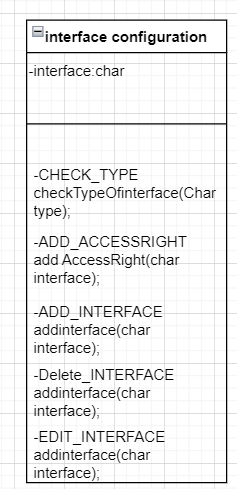
\includegraphics[width=0.3\linewidth]{picture/3-4/3-4-4.png}
    \caption{Interface Configuration}
    \label{fig:enter-label}
\end{figure}

\textbf{Explanations}
\begin{itemize}
    \item \texttt{- interface: char} is the interface of interface configuration
    \item \texttt{- CHECK\_TYPEcheckTypeOfinterface(char type)} is to check the type of the interface
    \item \texttt{- ADD\_INTERFACEaddInterface(char interface)} is to add a new interface that needs to be configured
    \item \texttt{- DELETE\_INTERFACEdeleteInterface(char interface)} is to delete the interface
    \item \texttt{- EDIT\_INTERFACEeditInterface(char interface)} is to edit the interface that needs to be configured
    \item \texttt{- ADD\_ACCESSRIGHTaddAccessRight()} is to add the right for users to access the interface
\end{itemize}

\textbf{Constraints} \\
TBD

\section{Data}

\subsection{Data User}

\begin{figure}[H]
    \centering
    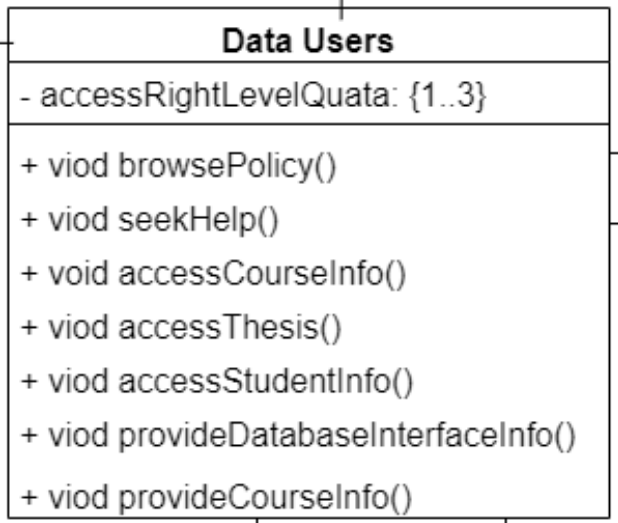
\includegraphics[width=0.3\linewidth]{picture/3-6/3-6-1.jpg}
    \caption{Data User}
    \label{fig:enter-label}
\end{figure}

\textbf{Explanations}
\begin{itemize}
    \item Access Right Level Quota has 3 levels:
    \begin{itemize}
        \item Public data access (access right level: 1)
        \item Private data consumption (access right level: 2)
        \item Private data provision (access right level: 3)
    \end{itemize}
    \item \texttt{browsePolicy()}, \texttt{seekHelp()}, \texttt{accessCourseInfo()}, \texttt{accessThesis()}, \texttt{accessStudentInfo()},\\ \texttt{provideDatabaseInterfaceInfo()}, \texttt{provideCourseInfo()} are the functions for data users.
\end{itemize}

\textbf{Constraints}
\begin{itemize}
    \item For the \texttt{provideDatabaseInterfaceInfo} method:
    \begin{itemize}
        \item \textbf{Pre-condition:} The user should be the data user.
        \item \textbf{Post-condition:} Open Database Info Interface.
    \end{itemize}
\end{itemize}

\subsection{User Question}

\begin{figure}[H]
    \centering
    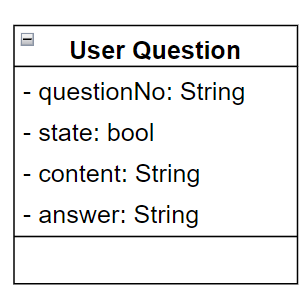
\includegraphics[width=0.3\linewidth]{picture/3-6/3-6-2.jpg}
    \caption{User Question}
    \label{fig:enter-label}
\end{figure}

\textbf{Explanations} \\
QuestionNo is the ID of the question for data user to check.

\textbf{Constraints} \\
None

\subsection{Activity Record (LOG)}

\begin{figure}[H]
    \centering
    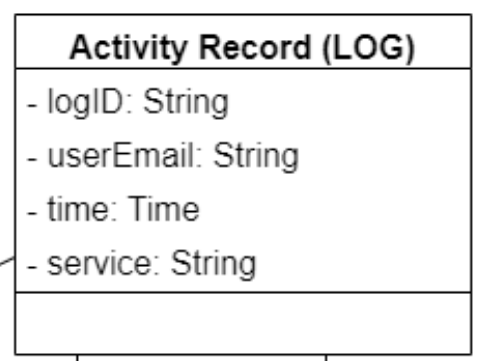
\includegraphics[width=0.3\linewidth]{picture/3-6/3-6-3.jpg}
    \caption{Activity Record (LOG)}
    \label{fig:enter-label}
\end{figure}

\textbf{Explanations} \\
logID is the ID of the activity record for data user to check.

\textbf{Constraints} \\
None


\section{Others}

\subsection{Email class}
\begin{figure}[H]
    \centering
    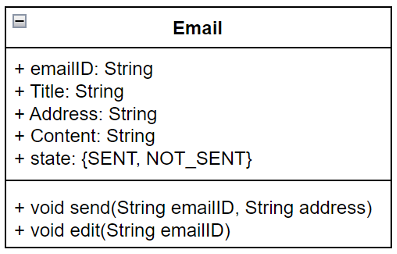
\includegraphics[width=0.5\linewidth]{picture/3-5/3-5-1.png}
    \caption{Email class}
    \label{fig:enter-label}
\end{figure}

\textbf{Explanations}
\begin{itemize}
    \item An email contains its \textbf{emailID}, title, address and content, while the state attribute of Email class represents whether the email is sent or not. 
    \item The \textbf{send()} operation would allow users to send the email with corresponding \textbf{emailID} to the corresponding address, while the \textbf{edit()} operation would allow users to edit the email with corresponding \textbf{emailID}. 
\end{itemize}

\textbf{Constraints}
\begin{itemize}
    \item For the \texttt{send} method:
    \begin{itemize}
        \item \textbf{Pre-condition:}
        \begin{itemize}
            \item state must be \texttt{NOT\_SENT}
            \item address and content must not be null
            \item address must be in a valid format
            \item the length of title must not be longer than the maximum length allowed
        \end{itemize}
        \item \textbf{Post-condition:}
        \begin{itemize}
            \item If the state is \texttt{SENT}, return \texttt{EMAIL\_ALREADY\_SENT}
            \item If the content is null, return \texttt{CONTENT\_CANNOT\_BE\_NULL}
            \item If the address does not exist, return \texttt{ADDRESS\_DOES\_NOT\_EXIST}
            \item If the length of title is longer than the maximum length allowed, return \texttt{TITLE\_SHOULD\_NOT\_LONGER\_THAN\_MAXIMUM}
            \item Otherwise, a new email is sent and return \texttt{SEND\_SUCCESSFUL}
        \end{itemize}
    \end{itemize}
\end{itemize}


\subsection{Data Sharing Policy class}
\begin{figure}[H]
    \centering
    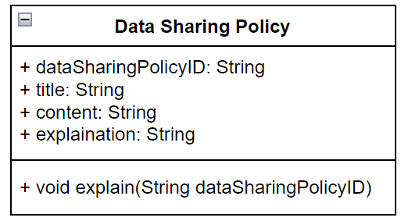
\includegraphics[width=0.5\linewidth]{picture/3-5/3-5-2.png}
    \caption{Data Sharing Policy Class}
    \label{fig:enter-label}
\end{figure}

\textbf{Explanations}

An data sharing policy contains \textbf{dataSharingPolicyID}, the title and content of the data sharing policy, while the \textbf{explanation} attribute of \textbf{DataSharingPolicy} class represents how E-Admin or Senior E-Admin explain the corresponding data sharing policy.

The \textbf{explain()} operation would let E-Admins and Senior E-Admins explain the data sharing policy with the corresponding \textbf{dataSharingPolicyID}.

\textbf{Constraints} \\
TBD

\subsection{Thesis class}

\begin{figure}[H]
    \centering
    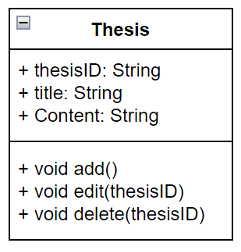
\includegraphics[width=0.5\linewidth]{picture/3-5/3-5-3.png}
    \caption{Thesis class}
    \label{fig:enter-label}
\end{figure}

\textbf{Explanations} \\
The \texttt{Thesis} class contains three attributes: the \textbf{thesisID}, the \textbf{title}, and the \texttt{content} of the thesis.

The \textbf{add()} operation would add a new thesis to the system, while the \textbf{edit()} and \textbf{delete()} operations could edit and delete the thesis with the corresponding \textbf{thesisID}, respectively.

\textbf{Constraints} \\
TBD

\subsection{Student Record class}
\begin{figure}[H]
    \centering
    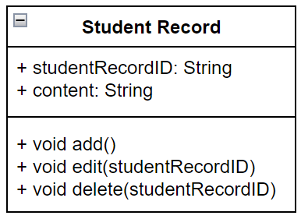
\includegraphics[width=0.5\linewidth]{picture/3-5/3-5-4.png}
    \caption{Student Record class}
    \label{fig:enter-label}
\end{figure}

\textbf{Explanations} \\
The \texttt{Student Record} class contains two attributes: the \textbf{studentRecordID} and the \textbf{content} of the student record.

The \textbf{add()} operation would add a new student record to the system, while the \textbf{edit()} and \textbf{delete()} operations could edit and delete the record with the corresponding \textbf{studentRecordID}, respectively.

\textbf{Constraints} \\
TBD

\subsection{Student Record List class}
\begin{figure}[H]
    \centering
    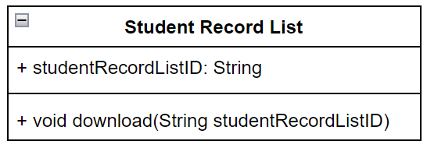
\includegraphics[width=0.5\linewidth]{picture/3-5/3-5-5.png}
    \caption{Student Record List class}
    \label{fig:enter-label}
\end{figure}

\textbf{Explanations} \\
The \texttt{StudentRecordList} class only has one attribute: the \textbf{studentRecordListID}, while one student record list contains one or more student records.

The \textbf{download()} operation would allow users to download the student record list from the system directly.

\textbf{Constraints} \\
TBD

\chapter{Alternative detailed design (Optional)}
None

\chapter{More considerations}
None
 
\nocite{*}
\printbibliography[heading=bibintoc]

\end{document}